\documentclass[11pt,a4paper]{article}
% Shared preamble for the NAIL094 reports
% Used by every task via % Shared preamble for the NAIL094 reports
% Used by every task via % Shared preamble for the NAIL094 reports
% Used by every task via \input{../../shared/preamble}

\usepackage[T1]{fontenc}
\usepackage[utf8]{inputenc}
\usepackage{lmodern}
\usepackage[margin=2.5cm]{geometry}

\usepackage{amsmath}
\usepackage{amssymb}
\usepackage{booktabs}
\usepackage{float}
\usepackage{graphicx}
\usepackage{listings}
\usepackage{xcolor}
\usepackage{caption}

\usepackage[hidelinks]{hyperref}

\setlength{\parskip}{0.5em}
\setlength{\parindent}{0pt}

% Title fields, set these in the report before \begin{document}
\makeatletter
\newcommand{\reportcourse}[1]{\def\@reportcourse{#1}}
\newcommand{\reporttask}[1]{\def\@reporttask{#1}}
\newcommand{\reportauthor}[1]{\def\@reportauthor{#1}}

\newcommand{\makereporttitle}{%
  \begin{center}
    {\LARGE\bfseries \@reportcourse \par}
    \vspace{0.8em}
    {\Large \@reporttask \par}
    \vspace{0.6em}
    {\normalsize \@reportauthor \par}
  \end{center}
  \vspace{1em}
  \hrule
  \vspace{1.5em}
}
\makeatother

% Inline code
\newcommand{\code}[1]{\texttt{#1}}

% Code listings
\lstdefinestyle{reportcode}{
  basicstyle=\ttfamily\small,
  keywordstyle=\color{blue!60!black},
  commentstyle=\color{gray},
  stringstyle=\color{green!40!black},
  breaklines=true,
  showstringspaces=false,
  frame=single,
  rulecolor=\color{gray!40},
  numbers=none,
}
\lstset{style=reportcode}


\usepackage[T1]{fontenc}
\usepackage[utf8]{inputenc}
\usepackage{lmodern}
\usepackage[margin=2.5cm]{geometry}

\usepackage{amsmath}
\usepackage{amssymb}
\usepackage{booktabs}
\usepackage{float}
\usepackage{graphicx}
\usepackage{listings}
\usepackage{xcolor}
\usepackage{caption}

\usepackage[hidelinks]{hyperref}

\setlength{\parskip}{0.5em}
\setlength{\parindent}{0pt}

% Title fields, set these in the report before \begin{document}
\makeatletter
\newcommand{\reportcourse}[1]{\def\@reportcourse{#1}}
\newcommand{\reporttask}[1]{\def\@reporttask{#1}}
\newcommand{\reportauthor}[1]{\def\@reportauthor{#1}}

\newcommand{\makereporttitle}{%
  \begin{center}
    {\LARGE\bfseries \@reportcourse \par}
    \vspace{0.8em}
    {\Large \@reporttask \par}
    \vspace{0.6em}
    {\normalsize \@reportauthor \par}
  \end{center}
  \vspace{1em}
  \hrule
  \vspace{1.5em}
}
\makeatother

% Inline code
\newcommand{\code}[1]{\texttt{#1}}

% Code listings
\lstdefinestyle{reportcode}{
  basicstyle=\ttfamily\small,
  keywordstyle=\color{blue!60!black},
  commentstyle=\color{gray},
  stringstyle=\color{green!40!black},
  breaklines=true,
  showstringspaces=false,
  frame=single,
  rulecolor=\color{gray!40},
  numbers=none,
}
\lstset{style=reportcode}


\usepackage[T1]{fontenc}
\usepackage[utf8]{inputenc}
\usepackage{lmodern}
\usepackage[margin=2.5cm]{geometry}

\usepackage{amsmath}
\usepackage{amssymb}
\usepackage{booktabs}
\usepackage{float}
\usepackage{graphicx}
\usepackage{listings}
\usepackage{xcolor}
\usepackage{caption}

\usepackage[hidelinks]{hyperref}

\setlength{\parskip}{0.5em}
\setlength{\parindent}{0pt}

% Title fields, set these in the report before \begin{document}
\makeatletter
\newcommand{\reportcourse}[1]{\def\@reportcourse{#1}}
\newcommand{\reporttask}[1]{\def\@reporttask{#1}}
\newcommand{\reportauthor}[1]{\def\@reportauthor{#1}}

\newcommand{\makereporttitle}{%
  \begin{center}
    {\LARGE\bfseries \@reportcourse \par}
    \vspace{0.8em}
    {\Large \@reporttask \par}
    \vspace{0.6em}
    {\normalsize \@reportauthor \par}
  \end{center}
  \vspace{1em}
  \hrule
  \vspace{1.5em}
}
\makeatother

% Inline code
\newcommand{\code}[1]{\texttt{#1}}

% Code listings
\lstdefinestyle{reportcode}{
  basicstyle=\ttfamily\small,
  keywordstyle=\color{blue!60!black},
  commentstyle=\color{gray},
  stringstyle=\color{green!40!black},
  breaklines=true,
  showstringspaces=false,
  frame=single,
  rulecolor=\color{gray!40},
  numbers=none,
}
\lstset{style=reportcode}


\reportcourse{NAIL094 --- Decision Procedures and SAT/SMT Solvers}
\reporttask{N-Queens Puzzle}
\reportauthor{Zerina Ahmetovic}

\begin{document}
\makereporttitle

\section{Task overview}

The $n$-queens puzzle~\cite{queens} is the problem of placing $n$ queens on an
$n \times n$
chessboard such that no two queens attack each other. The task is to model
the puzzle as a satisfiability problem, solve it with at least three
different solvers, and measure the performance (ex. the maximum value of 
$n$ for which each SAT or SMT solver solves the problem within a minute).

\section{Analysis}

\subsection*{Variables}

For a board of size $n$ there is one Boolean variable per square,
$x_{r,c}$, which is true only when a queen stands on row $r$ and column $c$.
Rows and columns are $0$-based, while DIMACS variables start at $1$, so the
squares are numbered row by row:
\[
  \mathrm{var}(r,c) = r \cdot n + c + 1 .
\]

\subsection*{Constraints}

The problem can be modelled using the following constraints:
\begin{itemize}
  \item at most one queen per row,
  \item at least one queen per column,
  \item at most one queen per diagonal, in both directions.
\end{itemize}

Throughout, $i$ denotes a row index and $j$ and $k$ denote column indices,
all of them ranging over $\{0, \dots, n-1\}$.

At most one is encoded pairwise. For a single fixed row $i$, forbidding two
queens in that row means forbidding them in every pair of distinct columns
$j$ and $k$, which gives one clause per pair:
\[
  \bigwedge_{0 \le j < k \le n-1}
  \left( \neg x_{i,j} \vee \neg x_{i,k} \right).
\]
The condition $j < k$ takes each unordered pair of columns once, since
$\{j,k\}$ and $\{k,j\}$ describe the same pair and would otherwise produce
the same clause twice. Every row must satisfy this, so the constraint for
the whole board is the conjunction over all rows:
\[
  \bigwedge_{i=0}^{n-1} \ \bigwedge_{0 \le j < k \le n-1}
  \left( \neg x_{i,j} \vee \neg x_{i,k} \right).
\]

At least one is a single clause per group. For a fixed column $j$, requiring
a queen somewhere in that column is the disjunction over all rows $i$, and
again every column must satisfy it, so the constraint for the whole board is
\[
  \bigwedge_{j=0}^{n-1} \ \bigvee_{i=0}^{n-1} x_{i,j}.
\]

The at most one constraints forbid queens from sharing a row or a
diagonal, following the rules of the game. Columns are left out on purpose, and
the counting argument below shows why the rules of the game still hold without
them. However, every one of them is satisfied by the empty board.
At least one rule solves this issue, forcing the $n$ queens to fill up $n$ rows.
With at least one queen in each of the $n$
columns there are at least $n$ queens on the board, and with at most one in
each of the $n$ rows there are at most $n$. So there are exactly $n$, every
row holds exactly one and every column holds exactly one. Adding at most one
per column or at least one per row would therefore be redundant, and by the
symmetry of rows and columns the choice of which one to limit to at least one is arbitrary.

\subsection*{Diagonals}

Fix a square $(i,j)$, where $i$ is its row and $j$ its column, and let $C$
be a non-zero integer, the offset along the diagonal. Moving $C$ steps down
and $C$ steps right reaches the square $(i+C,\, j+C)$, which lies on the
same descending diagonal, and moving $C$ steps down and $C$ steps left
reaches $(i+C,\, j-C)$, which lies on the same ascending diagonal. The
offset $C$ is admissible only when the square it reaches is still on the
board, that is when
\[
  0 \le i+C \le n-1
  \quad\text{and}\quad
  0 \le j+C \le n-1
\]
in the descending case, and $0 \le i+C \le n-1$ together with
$0 \le j-C \le n-1$ in the ascending case. The case $C = 0$ is excluded
as it returns the reference square.

Two queens attack each other diagonally when one is reached from the
other in one of these two ways, so the constraint is
\[
  \bigwedge_{i,j} \ \bigwedge_{C \neq 0}
  \left( \neg x_{i,j} \vee \neg x_{i+C,\,j+C} \right)
  \quad\text{and}\quad
  \bigwedge_{i,j} \ \bigwedge_{C \neq 0}
  \left( \neg x_{i,j} \vee \neg x_{i+C,\,j-C} \right),
\]
taken over every square $(i,j)$ of the board and every admissible $C$.

For the code implementation the same constraint is stated more conveniently.
Any two squares $(r_1,c_1)$ and $(r_2,c_2)$ related by the descending offset
satisfy $r_1 - c_1 = r_2 - c_2$, and any two related by the ascending offset
satisfy $r_1 + c_1 = r_2 + c_2$. A whole diagonal is therefore the set of
squares on which one of these two quantities is constant. Writing $d$ for
the constant value of $r-c$ and $s$ for the constant value of $r+c$, the
diagonals are
\[
  D_d = \{\, (r,c) : r - c = d \,\},
  \qquad d = -(n-1), \dots, n-1,
\]
\[
  S_s = \{\, (r,c) : r + c = s \,\},
  \qquad s = 0, \dots, 2n-2,
\]
which is $2n-1$ groups in each direction, $4n-2$ in total. Applying at most
one to every group $D_d$ and every group $S_s$ gives the same set of clauses
as the formulation above. It is preferable in code for two reasons: each
pair is generated once instead of twice, since iterating over squares and
offsets reaches the pair $\{(i,j), (i+C,j+C)\}$ once from each of its two
squares, and a group is a plain list of literals that can be handed to any
at most one encoding. Groups containing a single square, which are the four
corners of the board, are skipped as they contain no pair.

There is no at least one constraint for the diagonals. There are $4n-2$
diagonals but only $n$ queens, so most of them are necessarily empty.

\subsection*{Encoding size}

\begin{table}[H]
\centering
\begin{tabular}{rrr}
\toprule
$n$ & variables & clauses \\
\midrule
8   & 64     & 512 \\
16  & 256    & 4\,416 \\
32  & 1\,024 & 36\,736 \\
64  & 4\,096 & 299\,776 \\
100 & 10\,000 & 1\,151\,800 \\
150 & 22\,500 & 3\,903\,950 \\
200 & 40\,000 & 9\,273\,600 \\
250 & 62\,500 & 18\,135\,750 \\
300 & 90\,000 & 31\,365\,400 \\
350 & 122\,500 & 49\,837\,550 \\
\bottomrule
\end{tabular}
\caption{Size of the pairwise encoding.}
\label{tab:size}
\end{table}

The number of variables in Table~\ref{tab:size} is $n^2$ by construction,
one per square. The number of clauses grows as $n^3$: there are $O(n)$
groups of size $O(n)$, and the pairwise encoding turns each group into
$O(n^2)$ clauses. The last column of the table confirms this, since the
ratio of clauses to $n^3$ settles at about $1.16$.
The practical consequence is that the encoding becomes large quickly, with over
$18$ million clauses at $n=250$ and almost $50$ million at $n=350$. This does
not affect the three solvers equally. Table~\ref{tab:times} shows that
Glucose and CaDiCaL run out of time inside their own search, so the size of
the formula is not what stops them, while MiniSat is fast enough that the
cost of building and loading the clauses is what ends its measurements
rather than the difficulty of the board.

\subsection*{Correctness}

The encoding was validated without a solver by enumerating all $2^{n^2}$
assignments for $n \le 4$ and comparing the number of models to the known
solution counts $1, 0, 0, 2$, and by checking for $n \le 7$ that every
non-attacking placement satisfies the formula. Two further checks were made:
that placements containing an attack are rejected, and that the diagonal
groups cover exactly the pairs of squares that attack each other
diagonally. Every model produced in the experiments was additionally decoded
and checked by an independent verifier, which re-derives the rules from the
board rather than from the encoding.

\section{Performance analysis}

\subsection*{Solvers}

Three solvers were used through the PySAT toolkit~\cite{pysat}: CaDiCaL
1.5.3~\cite{cadical}, Glucose 4~\cite{glucose} and MiniSat
2.2~\cite{minisat}, which PySAT identifies as \code{cadical153},
\code{glucose4} and \code{minisat22} respectively.

\subsection*{Setup}

All measurements were taken on a single local machine, an Intel Core
i7-13700H with 16\,GB of memory running Windows 11, under Python 3.11.9
with python-sat 1.9.dev7. Each instance was solved in its own process with a
\textasciitilde{} 60 second budget. Three phases were timed separately: building the clause
list in Python, loading the clauses into the solver, and the search itself.
Only the last two are the work of the solver, while the first is the cost of the Python implementation (hence the separation).

\subsection*{Running time}

\begin{table}[H]
\centering
\begin{tabular}{rlrrrr}
\toprule
$n$ & solver & encode [s] & load [s] & solve [s] & total [s] \\
\midrule
8   & cadical153 & 0.001 & 0.001 & 0.000 & 0.002 \\
8   & glucose4   & 0.001 & 0.008 & 0.002 & 0.011 \\
8   & minisat22  & 0.003 & 0.000 & 0.001 & 0.004 \\
16  & cadical153 & 0.002 & 0.004 & 0.060 & 0.065 \\
16  & glucose4   & 0.003 & 0.003 & 0.005 & 0.010 \\
16  & minisat22  & 0.002 & 0.002 & 0.002 & 0.006 \\
32  & cadical153 & 0.009 & 0.018 & 0.376 & 0.403 \\
32  & glucose4   & 0.007 & 0.015 & 9.918 & 9.940 \\
32  & minisat22  & 0.009 & 0.016 & 0.004 & 0.030 \\
64  & cadical153 & 0.108 & 0.138 & 0.911 & 1.157 \\
64  & glucose4   & 0.089 & 0.137 & 0.013 & 0.238 \\
64  & minisat22  & 0.118 & 0.128 & 0.016 & 0.262 \\
100 & cadical153 & 0.525 & 0.542 & 2.218 & 3.285 \\
100 & glucose4   & 0.521 & \multicolumn{3}{c}{timeout} \\
100 & minisat22  & 0.548 & 0.466 & 0.027 & 1.040 \\
150 & cadical153 & 1.951 & 2.811 & 15.307 & 20.069 \\
150 & minisat22  & 1.965 & 2.167 & 0.184 & 4.317 \\
200 & cadical153 & 4.602 & 4.123 & 13.956 & 22.682 \\
200 & minisat22  & 4.334 & 3.551 & 0.119 & 8.005 \\
250 & cadical153 & 8.578 & 8.384 & 34.658 & 51.620 \\
250 & minisat22  & 8.524 & 7.025 & 0.508 & 16.057 \\
300 & cadical153 & 13.752 & \multicolumn{3}{c}{timeout} \\
300 & minisat22  & 15.109 & 22.936 & 0.928 & 38.973 \\
350 & minisat22  & 46.746 & \multicolumn{3}{c}{timeout} \\
\bottomrule
\end{tabular}
\caption{Running time in seconds. Encoding is Python work, loading and
solving are the solver. A timeout marks a run stopped at the 60 second
budget, which is applied to loading and solving together. Encoding is not
counted against it, and a solver is not tried on larger boards once it has
timed out.}
\label{tab:times}
\end{table}

Table~\ref{tab:times} separates the three solvers. MiniSat is the
fastest throughout, needing about half a second of search at $n=250$ and
under one second at $n=300$, while CaDiCaL needs roughly $35$ seconds for
$n=250$ and does not finish $n=300$. Glucose is the weakest and already
fails at $n=100$. The encode and load columns are almost identical across
solvers at the same $n$, as expected, since the same clause list is built
and handed over in every case. What they show is their size relative to the
solve column: at $n=300$ MiniSat spends $0.928$ seconds
searching out of $38.973$ seconds in total, so under three percent of its
time is spent solving and the rest goes on constructing and transferring the
formula.

The last row is the clearest illustration of this. At $n=350$ the encoding
alone took $46.746$ seconds, and loading the resulting $49.8$ million
clauses into MiniSat did not finish within the budget, so the run was
stopped before the search began. MiniSat did not fail to solve that board,
it never got the chance to try.

\begin{table}[H]
\centering
\begin{tabular}{lrrr}
\toprule
solver & search only & search + loading & incl. encoding \\
\midrule
cadical153 & 250 & 250 & 250 \\
glucose4   & 64  & 64  & 64 \\
minisat22  & 300 & 300 & 300 \\
\bottomrule
\end{tabular}
\caption{Largest $n$ handled within a budget of 60 seconds, under three
different definitions of what is being timed.}
\label{tab:maxn}
\end{table}

Table~\ref{tab:maxn} gives the same limit under three definitions of the
budget, and the three agree for every solver, so the choice of definition
does not change the answer at these sizes. Each value is the largest board
tested before that solver first exceeded the budget, since the sweep retires
a solver at its first timeout and does not try it again on a larger board.
That is a weaker statement than a limit of the solver. Running time does not
grow steadily with $n$, as Table~\ref{tab:nonmono} shows, so a solver that
fails at one size may well succeed at a larger one, and the figures below are
best read as the point where each solver first ran out of budget.

The three limits do not all mean the same thing, however. Glucose and
CaDiCaL reached limits of their search: Glucose spent nearly the whole
budget searching at $n=100$ after solving $n=64$ in $13$ milliseconds, and
CaDiCaL already needed $34.658$ seconds of search at $n=250$, so it had
little room left at $n=300$. MiniSat did not. Its search at $n=300$ took
$0.928$ seconds, and the run at $n=350$ was stopped while the clauses were
still being loaded. Its value of $300$ therefore measures how large a
formula could be built and transferred in the time available, not how large
a board it can solve.

\begin{figure}[H]
\centering
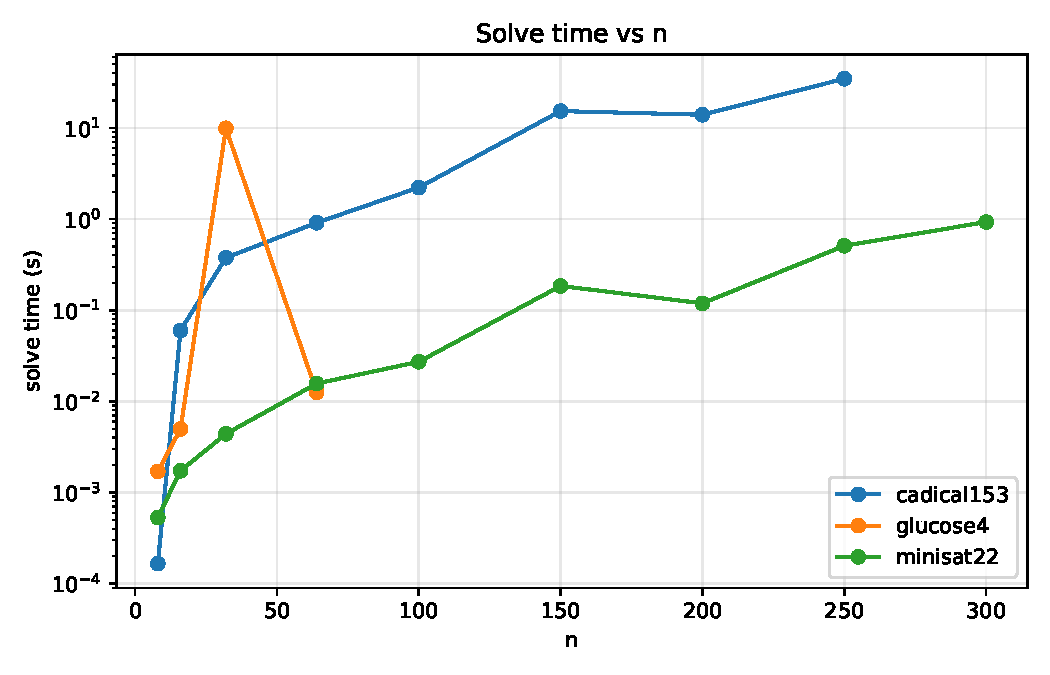
\includegraphics[width=0.72\textwidth]{figures/solve_time.pdf}
\caption{Search time against $n$, logarithmic scale.}
\label{fig:solvetime}
\end{figure}

Figure~\ref{fig:solvetime} shows the same measurements as
Table~\ref{tab:times} and makes the gap between the solvers easier to see.
The vertical axis is logarithmic, so the roughly constant vertical distance
between the MiniSat and CaDiCaL curves at larger $n$ means a constant
factor rather than a constant difference in seconds: CaDiCaL is $83$ times
slower at $n=150$, $117$ times at $n=200$ and $68$ times at $n=250$. The
Glucose curve is the irregular one, rising sharply at $n=32$ and dropping
again at $n=64$ before it times out.

\subsection*{Solver statistics}

\begin{table}[H]
\centering
\begin{tabular}{rlrrrr}
\toprule
$n$ & solver & restarts & conflicts & decisions & propagations \\
\midrule
8   & cadical153 & 0 & 15 & 25 & 341 \\
8   & glucose4   & 1 & 289 & 403 & 3\,541 \\
8   & minisat22  & 2 & 117 & 205 & 1\,938 \\
16  & cadical153 & 78 & 3\,857 & 5\,126 & 129\,513 \\
16  & glucose4   & 2 & 490 & 1\,067 & 9\,654 \\
16  & minisat22  & 3 & 206 & 640 & 6\,541 \\
32  & cadical153 & 303 & 10\,020 & 13\,879 & 793\,327 \\
32  & glucose4   & 3 & 100\,025 & 121\,448 & 2\,448\,651 \\
32  & minisat22  & 3 & 221 & 2\,014 & 13\,758 \\
64  & cadical153 & 257 & 10\,020 & 16\,804 & 2\,088\,977 \\
64  & glucose4   & 3 & 340 & 8\,682 & 35\,816 \\
64  & minisat22  & 4 & 414 & 10\,180 & 48\,240 \\
100 & cadical153 & 297 & 11\,377 & 28\,233 & 3\,590\,037 \\
100 & minisat22  & 4 & 414 & 26\,010 & 96\,182 \\
150 & cadical153 & 370 & 15\,069 & 65\,018 & 8\,511\,212 \\
150 & minisat22  & 5 & 512 & 76\,352 & 252\,736 \\
200 & cadical153 & 381 & 15\,345 & 124\,769 & 11\,581\,979 \\
200 & minisat22  & 5 & 531 & 132\,618 & 363\,383 \\
250 & cadical153 & 814 & 16\,889 & 211\,418 & 23\,284\,404 \\
250 & minisat22  & 10 & 1\,442 & 327\,742 & 870\,972 \\
300 & minisat22  & 7 & 809 & 383\,627 & 1\,152\,103 \\
\bottomrule
\end{tabular}
\caption{Counters reported by the solvers. These are counts, and machine independent.}
\label{tab:stats}
\end{table}

The counters in Table~\ref{tab:stats} compare the same solvers by accessing
PySAT's built in method \code{accum\_stats()}, and they agree with the
running times. At $n=200$ the two
remaining solvers make a comparable number of decisions, about $125$ and
$133$ thousand, but CaDiCaL performs roughly thirty times as many
propagations and about thirty times as many conflicts. Glucose is the
extreme case: at $n=32$ it records over $100$ thousand conflicts against
MiniSat's $221$, which accounts for the $9.918$ seconds it spent on that
board in Table~\ref{tab:times}.

\begin{figure}[H]
\centering
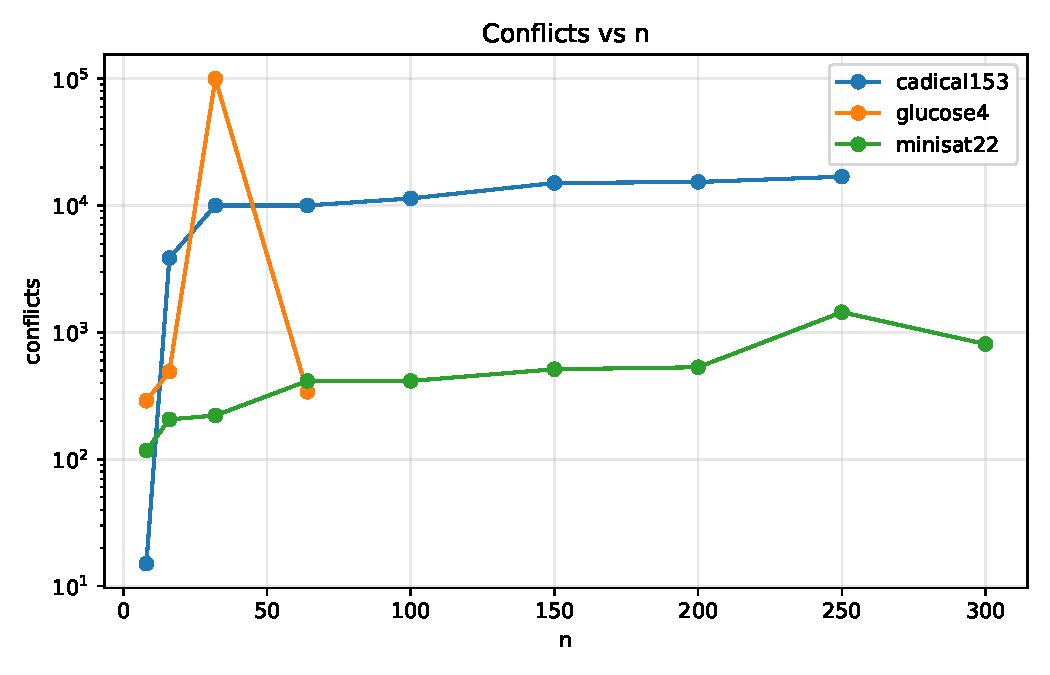
\includegraphics[width=0.72\textwidth]{figures/conflicts.pdf}
\caption{Conflicts against $n$, logarithmic scale.}
\label{fig:conflicts}
\end{figure}

Figure~\ref{fig:conflicts} plots the conflict counts of
Table~\ref{tab:stats} and has almost the same shape as
Figure~\ref{fig:solvetime}, which confirms that the differences in running
time come from how much search each solver performs and not from the
measurement conditions. The MiniSat curve stays low and nearly flat, while
the spike in the Glucose curve at $n=32$ matches its spike in running time.

\subsection*{Non-monotonicity}

\begin{table}[H]
\centering
\begin{tabular}{lrrr}
\toprule
solver & smaller board & larger board & speedup \\
\midrule
glucose4   & $n=32$, 9.918\,s  & $n=64$, 0.013\,s  & $791\times$ \\
minisat22  & $n=150$, 0.184\,s & $n=200$, 0.119\,s & $1.55\times$ \\
cadical153 & $n=150$, 15.307\,s & $n=200$, 13.956\,s & $1.10\times$ \\
\bottomrule
\end{tabular}
\caption{Cases where a larger board was solved faster than a smaller one.}
\label{tab:nonmono}
\end{table}

Table~\ref{tab:nonmono} records every case where increasing the board size
made the search easier rather than harder, and it happened to all three
solvers. The effect is small for MiniSat and CaDiCaL, which both solved
$n=200$ slightly faster than $n=150$, but extreme for Glucose, which needed
almost ten seconds for $n=32$ and only thirteen milliseconds for $n=64$, a
board four times larger. Running time therefore does not grow steadily with
$n$, which is worth keeping in mind when reading a single figure such as the
largest $n$ solved within a minute.

\subsection*{Code}

All code is in \code{n-queens/code/} and is available in the
repository~\cite{repo}.

\begin{itemize}
  \item \code{nqueens.py} is the main module in which the encoding is. It maps
  a square to its variable index, collects the literals of every row, column
  and diagonal into groups, applies at most one (AMO) or at least one (ALO) to each
  group, and returns the resulting clause list. It also decodes a model back
  into a board, verifies a board independently of the encoding, and writes
  the formula in DIMACS format. As it does not import any solver, it can be independently
  used and tested.

  \item \code{bench.py} runs the measurements. Each instance is solved in
  its own child process, so the 60 second budget can be enforced by
  terminating it, and the three phases of encoding, loading and
  searching are timed separately. It also collects the solver counters and
  sweeps over a list of board sizes, dropping a solver once it exceeds the
  set budget.

  \item \code{test\_queens.py} validates the encoding without using a
  solver, by enumerating all assignments for small boards, comparing the
  number of models against the known solution counts, and checking that the
  diagonal groups cover exactly the diagonally attacking pairs.

  \item \code{experiments.ipynb} produces everything shown in this report.
  It imports the two modules above, runs the checks and the sweep, and
  writes out the tables, the figures in \code{report/figures/}, and the two
  result files.

  \item \code{results.csv} and \code{stats.csv} store the output of the
  sweep, the first with the timings and the second with the solver counters.
\end{itemize}

\subsection*{Summary}

The three solvers are far apart on the hierarchy when tested on NQueens problem instance.
MiniSat was the fastest at every board size, finishing
$n=300$ in under one second of search. CaDiCaL, a recent competition winner,
needed $34.658$ seconds for $n=250$ and did not finish $n=300$, making it
between $68$ and $117$ times slower than MiniSat depending on the board.
Glucose was the weakest and failed already at $n=100$. The counters in
Table~\ref{tab:stats} rule out the machine as an explanation, since they are
counts rather than times and reproduce exactly across runs: at $n=200$
CaDiCaL performed roughly thirty times as many propagations and conflicts as
MiniSat, in the same proportion as the measured times.

The second finding is that for the fastest solver the
encoding, not the search, is what ends the experiment. At $n=300$ MiniSat
spent $0.928$ seconds searching out of $38.973$ seconds in total, so under
three percent of the work was solving and the rest was building the clause
list in Python and transferring it into the solver. At $n=350$ the encoding
alone took $46.746$ seconds and the clauses could not even be loaded within
the budget, so the search never started. This follows directly from the
pairwise encoding growing as $n^3$, reaching almost $50$ million clauses at
$n=350$. A more compact encoding of the at most one constraint would be the
first thing to change before attempting larger boards.

The three ceilings in Table~\ref{tab:maxn} therefore have to be read
differently even though they were all measured the same way. Glucose and
CaDiCaL stopped because their search ran out of time, so $64$ and $250$
describe the solvers. MiniSat stopped because the formula could no longer be
prepared in time, so $300$ describes the encoding and the machine rather
than the solver, and its true limit is somewhere above it.

Finally, running time does not grow steadily with $n$, and this affected all
three solvers. Glucose solved $n=64$ about $791$ times faster than $n=32$
despite the larger board having four times as many squares, and both MiniSat
and CaDiCaL solved $n=200$ faster than $n=150$. A single measurement at one
board size is therefore a weak description of a solver, and the shape of the
whole curve in Figure~\ref{fig:solvetime} provides more insight into this matter.

\clearpage

\begin{thebibliography}{9}

\bibitem{queens}
Wikipedia, \emph{Eight queens puzzle}.
\url{https://en.wikipedia.org/wiki/Eight_queens_puzzle}

\bibitem{pysat}
A. Ignatiev, A. Morgado, J. Marques-Silva,
\emph{PySAT: A Python Toolkit for Prototyping with SAT Oracles}, SAT 2018.
\url{https://pysathq.github.io}

\bibitem{cadical}
A. Biere, \emph{CaDiCaL}.
\url{http://fmv.jku.at/cadical}

\bibitem{glucose}
G. Audemard, L. Simon, \emph{Glucose}.
\url{https://www.labri.fr/perso/lsimon/glucose}

\bibitem{minisat}
N. E{\'e}n, N. S{\"o}rensson, \emph{MiniSat}.
\url{http://minisat.se}

\bibitem{repo}
Z. Ahmetovic, source code for this task.
\url{https://github.com/inferno73/SAT-solver-NAIL094}

\end{thebibliography}

\end{document}


